\newcommand{\gptpart}{29}
\newcommand{\gpttitle}{Experimental Divergence}
\newcommand{\gptsubtitle}{Where the Accounts Part Ways, and How to Tell Them Apart}
\newcommand{\gptdate}{November 2026}
% Shared preamble for the second edition of Graviton Pressure Theory.
% A part's own file sets \gptpart, \gpttitle, \gptsubtitle and \gptdate, then % Shared preamble for the second edition of Graviton Pressure Theory.
% A part's own file sets \gptpart, \gpttitle, \gptsubtitle and \gptdate, then % Shared preamble for the second edition of Graviton Pressure Theory.
% A part's own file sets \gptpart, \gpttitle, \gptsubtitle and \gptdate, then \input{../common/preamble}.
\documentclass[11pt,a4paper]{article}
\usepackage[T1]{fontenc}
\usepackage[utf8]{inputenc}
\usepackage{mathpazo}
\usepackage[scaled=0.92]{helvet}
\usepackage{amsmath,amssymb}
\usepackage[margin=2.5cm]{geometry}
\usepackage{microtype}
\usepackage{graphicx}
\usepackage{booktabs,array,tabularx}
\usepackage[font=small,labelfont=bf]{caption}
\usepackage{enumitem}
\usepackage[authoryear,round]{natbib}
\usepackage{titlesec}
\usepackage[titles]{tocloft}
\renewcommand{\cftsecfont}{\bfseries}\renewcommand{\cftsecpagefont}{\bfseries}
\renewcommand{\cftsecleader}{\hfill}\setlength{\cftsecnumwidth}{3.2em}
\usepackage{gpt-status}
\usepackage[hidelinks]{hyperref}
\setlength{\parskip}{4pt}
\setlength{\emergencystretch}{3em}
\setlength{\parindent}{0pt}
\setlist{itemsep=2pt,topsep=3pt}
\titleformat{\section}{\Large\bfseries}{\thesection}{1em}{}
\titleformat{\subsection}{\large\bfseries}{\thesubsection}{1em}{}
\renewcommand{\thesection}{\gptpart.\arabic{section}}
\renewcommand{\thetable}{\gptpart.\arabic{table}}
\renewcommand{\thefigure}{\gptpart.\arabic{figure}}
\renewcommand{\theequation}{\gptpart.\arabic{equation}}
\setcounter{tocdepth}{1}
\makeatletter\renewcommand{\@pnumwidth}{2.2em}\renewcommand{\@tocrmarg}{3em}
\makeatother
\bibliographystyle{plainnat}
\newcommand{\gptitle}{%
  \begin{titlepage}\centering
  \vspace*{3cm}
  {\Huge\bfseries Graviton Pressure Theory\par}\vspace{0.8cm}
  {\Large The Unified Framework\par}\vspace{0.2cm}
  {\large Individual Submission\par}\vspace{0.6cm}
  {\normalsize This document is part of a multi-part scientific framework\par}\vspace{2cm}
  {\normalsize Part \gptpart\ of 30\par}\vspace{0.8cm}
  {\huge\bfseries \gpttitle\par}\vspace{0.6cm}
  {\Large \gptsubtitle\par}\vspace{1.5cm}
  {\small\begin{minipage}{0.75\textwidth}\centering This submission is part of the broader Graviton Pressure Theory (GPT) project, a redefinition of gravitational interaction rooted in causal field dynamics and physical force transmission. Each document is designed to stand on its own; its full context emerges as part of the larger framework. For the complete series, see https://peopleoftheworld.net/graviton-pressure-theory/.\end{minipage}\par}
  \vfill
  {\large Author: Shareef Ali Rashada\par}\vspace{0.2cm}
  {\normalsize shareef@peopleoftheworld.net\par}\vspace{0.5cm}
  {\normalsize Second edition, \gptdate\par}
  \end{titlepage}
  \setcounter{page}{1}\tableofcontents\clearpage}
.
\documentclass[11pt,a4paper]{article}
\usepackage[T1]{fontenc}
\usepackage[utf8]{inputenc}
\usepackage{mathpazo}
\usepackage[scaled=0.92]{helvet}
\usepackage{amsmath,amssymb}
\usepackage[margin=2.5cm]{geometry}
\usepackage{microtype}
\usepackage{graphicx}
\usepackage{booktabs,array,tabularx}
\usepackage[font=small,labelfont=bf]{caption}
\usepackage{enumitem}
\usepackage[authoryear,round]{natbib}
\usepackage{titlesec}
\usepackage[titles]{tocloft}
\renewcommand{\cftsecfont}{\bfseries}\renewcommand{\cftsecpagefont}{\bfseries}
\renewcommand{\cftsecleader}{\hfill}\setlength{\cftsecnumwidth}{3.2em}
\usepackage{gpt-status}
\usepackage[hidelinks]{hyperref}
\setlength{\parskip}{4pt}
\setlength{\emergencystretch}{3em}
\setlength{\parindent}{0pt}
\setlist{itemsep=2pt,topsep=3pt}
\titleformat{\section}{\Large\bfseries}{\thesection}{1em}{}
\titleformat{\subsection}{\large\bfseries}{\thesubsection}{1em}{}
\renewcommand{\thesection}{\gptpart.\arabic{section}}
\renewcommand{\thetable}{\gptpart.\arabic{table}}
\renewcommand{\thefigure}{\gptpart.\arabic{figure}}
\renewcommand{\theequation}{\gptpart.\arabic{equation}}
\setcounter{tocdepth}{1}
\makeatletter\renewcommand{\@pnumwidth}{2.2em}\renewcommand{\@tocrmarg}{3em}
\makeatother
\bibliographystyle{plainnat}
\newcommand{\gptitle}{%
  \begin{titlepage}\centering
  \vspace*{3cm}
  {\Huge\bfseries Graviton Pressure Theory\par}\vspace{0.8cm}
  {\Large The Unified Framework\par}\vspace{0.2cm}
  {\large Individual Submission\par}\vspace{0.6cm}
  {\normalsize This document is part of a multi-part scientific framework\par}\vspace{2cm}
  {\normalsize Part \gptpart\ of 30\par}\vspace{0.8cm}
  {\huge\bfseries \gpttitle\par}\vspace{0.6cm}
  {\Large \gptsubtitle\par}\vspace{1.5cm}
  {\small\begin{minipage}{0.75\textwidth}\centering This submission is part of the broader Graviton Pressure Theory (GPT) project, a redefinition of gravitational interaction rooted in causal field dynamics and physical force transmission. Each document is designed to stand on its own; its full context emerges as part of the larger framework. For the complete series, see https://peopleoftheworld.net/graviton-pressure-theory/.\end{minipage}\par}
  \vfill
  {\large Author: Shareef Ali Rashada\par}\vspace{0.2cm}
  {\normalsize shareef@peopleoftheworld.net\par}\vspace{0.5cm}
  {\normalsize Second edition, \gptdate\par}
  \end{titlepage}
  \setcounter{page}{1}\tableofcontents\clearpage}
.
\documentclass[11pt,a4paper]{article}
\usepackage[T1]{fontenc}
\usepackage[utf8]{inputenc}
\usepackage{mathpazo}
\usepackage[scaled=0.92]{helvet}
\usepackage{amsmath,amssymb}
\usepackage[margin=2.5cm]{geometry}
\usepackage{microtype}
\usepackage{graphicx}
\usepackage{booktabs,array,tabularx}
\usepackage[font=small,labelfont=bf]{caption}
\usepackage{enumitem}
\usepackage[authoryear,round]{natbib}
\usepackage{titlesec}
\usepackage[titles]{tocloft}
\renewcommand{\cftsecfont}{\bfseries}\renewcommand{\cftsecpagefont}{\bfseries}
\renewcommand{\cftsecleader}{\hfill}\setlength{\cftsecnumwidth}{3.2em}
\usepackage{gpt-status}
\usepackage[hidelinks]{hyperref}
\setlength{\parskip}{4pt}
\setlength{\emergencystretch}{3em}
\setlength{\parindent}{0pt}
\setlist{itemsep=2pt,topsep=3pt}
\titleformat{\section}{\Large\bfseries}{\thesection}{1em}{}
\titleformat{\subsection}{\large\bfseries}{\thesubsection}{1em}{}
\renewcommand{\thesection}{\gptpart.\arabic{section}}
\renewcommand{\thetable}{\gptpart.\arabic{table}}
\renewcommand{\thefigure}{\gptpart.\arabic{figure}}
\renewcommand{\theequation}{\gptpart.\arabic{equation}}
\setcounter{tocdepth}{1}
\makeatletter\renewcommand{\@pnumwidth}{2.2em}\renewcommand{\@tocrmarg}{3em}
\makeatother
\bibliographystyle{plainnat}
\newcommand{\gptitle}{%
  \begin{titlepage}\centering
  \vspace*{3cm}
  {\Huge\bfseries Graviton Pressure Theory\par}\vspace{0.8cm}
  {\Large The Unified Framework\par}\vspace{0.2cm}
  {\large Individual Submission\par}\vspace{0.6cm}
  {\normalsize This document is part of a multi-part scientific framework\par}\vspace{2cm}
  {\normalsize Part \gptpart\ of 30\par}\vspace{0.8cm}
  {\huge\bfseries \gpttitle\par}\vspace{0.6cm}
  {\Large \gptsubtitle\par}\vspace{1.5cm}
  {\small\begin{minipage}{0.75\textwidth}\centering This submission is part of the broader Graviton Pressure Theory (GPT) project, a redefinition of gravitational interaction rooted in causal field dynamics and physical force transmission. Each document is designed to stand on its own; its full context emerges as part of the larger framework. For the complete series, see https://peopleoftheworld.net/graviton-pressure-theory/.\end{minipage}\par}
  \vfill
  {\large Author: Shareef Ali Rashada\par}\vspace{0.2cm}
  {\normalsize shareef@peopleoftheworld.net\par}\vspace{0.5cm}
  {\normalsize Second edition, \gptdate\par}
  \end{titlepage}
  \setcounter{page}{1}\tableofcontents\clearpage}

\graphicspath{{figs/}}
\begin{document}
\gptitle

\section*{About This Paper}
\addcontentsline{toc}{section}{About This Paper}

Graviton Pressure Theory never argues against a measurement. Every result stands, and every part of the mechanism must pass it. This paper asks where the mechanism and the standard account expect different things, and how an experiment could tell them apart.

It does three things. It sets out what counts as a divergence, and what does not. It reads again the classroom demonstrations that are often taken as evidence for one account or the other, and says which of them can decide anything. And it gathers in one place the tests that Parts 9 to 28 have sent here: the experiments where GPT expects something the standard account does not, each with what is expected, what has been measured, and what result would count against GPT.

This is the second edition; what changed from the first is listed at the end. Claims are marked by their status, as the key shows.

\statuskey

\section{What a Divergence Is}

\subsection{Three kinds of difference}

\argm{Two accounts can differ in three ways, and only two of them can be settled by an experiment.}
\begin{itemize}
\item \textbf{The same outcome, read differently.} Both accounts give the same number, and differ in what they say causes it. Free fall, weight, the bending of light, the slowing of clocks and the turning of Mercury's orbit are all here: GPT reproduces the standard numbers and names a different mechanism (Parts 5 and 8).\fn{rashadaPart8} No experiment that measures only the outcome can choose between them; the choice rests on mechanism, on which account names what touches what. Most classroom demonstrations are of this kind.
\item \textbf{An effect the standard account does not address.} GPT expects something the standard account is silent on, or expects to be zero: a held body's weight depending on its structure, a spinning body leaving an imprint beyond its shape, a clock's slowing depending on its internal order. An experiment can look for these.
\item \textbf{A different number.} The two accounts expect different values for the same measurement. The clearest is the behaviour of gravity where the inflow's acceleration falls to about $1.2\times10^{-10}$ m/s$^2$: GPT's relaxation boundary, against the standard account's dark matter (Part 9).\fn{rashadaPart9}
\end{itemize}

\subsection{How a test is read}

\argm{A test of the whole mechanism and a test of one of its parts say different things.} An \emph{outcome test} measures a result directly, such as two materials falling alike to one part in $10^{15}$;\fn{touboul2022} it constrains every account, whatever its parts. A \emph{subset test} models some of the parts, and shows only that those parts alone do not produce the result. So each test below is stated with four things: what GPT expects, what the standard account expects, what has been measured, and what result would count against GPT.

\section{The Demonstrations, Read Again}

Many demonstrations are offered as showing that gravity is a pressure, or that it is not. Read with care, nearly all of them show the same outcome under both accounts. Their value is that they make the question of mechanism concrete; they cannot decide it. Table~\ref{tab:demos} reads each one again. Where a demonstration points to a real divergence, the table says where in Section~3 it is taken up.

\begin{table}[p]\centering\footnotesize
\caption{Demonstrations often cited for or against a pressure account of gravity, read again: what is seen, how each account reads it, and whether it can decide between them.}
\renewcommand{\arraystretch}{1.05}\begin{tabularx}{\linewidth}{@{}>{\raggedright\arraybackslash}p{0.18\linewidth} >{\raggedright\arraybackslash}p{0.22\linewidth} >{\raggedright\arraybackslash}X >{\raggedright\arraybackslash}p{0.09\linewidth}@{}}\toprule
\textbf{Demonstration} & \textbf{What is seen} & \textbf{The two readings} & \textbf{Decides?}\\\midrule
A robot arm holding a weight & the motors draw power while nothing moves; a shelf holding the same weight draws none & the motors' cost is their own design; GPT adds that the medium's momentum passes through the held weight without being used up (Part 6) & no\\
A magnet holding a washer & held indefinitely, with no input & standard: a static force; GPT: the delivery relayed, held by the magnet's organised swirl (Parts 6, 22) & no\\
A helium balloon in a dropped lift & the balloon stops rising and floats with the car & buoyancy needs the air's pressure to rise with depth; in a free fall the air is carried alike and that rise vanishes. Both accounts agree & no\\
Tension in a suspended mass & the rope carries the weight & GPT reads tension as a pressure deficit in the medium; its derivation is owed (Part 7) & no\\
A comb bending a stream of water & the stream bends toward the comb & induced charge; GPT names the medium's part in it (Part 11) & no\\
A gyroscope's precession & a torque turns the spin axis & both reproduce it; the Earth's spin carrying a gyroscope's axis is the frame dragging Gravity Probe B measured, the medium's swirl in GPT (Part 16) & no\\
A steel plate near a magnet & the plate turns into line before it moves & the magnet magnetises the plate most easily along its length, and the turning comes first; GPT reads it as the swirl organising the plate (Part 22) & no\\
An L-shaped body dropped & in air it turns as it drops & in a vacuum it does not: the delivery reaches every particle alike, so there is no turning force. In air the turning is drag. Whether a held body's centre of gravity moves from its centre of mass as it is turned is a real test (§\ref{sec:structure}) & held: yes\\
A heated body on a scale & the reading drifts & heat added raises mass by $\Delta E/c^2$, about $5\times10^{-13}$ for a kilogram of steel warmed 100 degrees; the drift seen is far larger, and is air rising off the warm body & no\\
Crystals in a row, the first set vibrating & a response at the last & through air or a mount, by sound. Across a vacuum, only the gravity of the moving mass, which is calculable; any excess would be GPT's (§\ref{sec:structure}) & in vacuum: yes\\
An actuator holding a load for hours & its power slowly rises & its windings warm, and their resistance rises; a shelf shows no cost at any time. Fatigue comes from changing loads (Part 6) & no\\
A body of quartz above foam, dropped & no tilt & different materials are carried alike, to one part in $10^{15}$ & no\\
A dense block and loose bearings of equal mass & they fall together & the same: delivery is in proportion to mass, not to packing & no\\
A crystal sheet between masses & no change in the force & gravity is not measurably shielded by matter (Part 15); a small shading at alignments remains a place to look (§\ref{sec:alignments}) & bounded\\
A hollow and a solid sphere of equal mass & they fall together & falling passes nothing from part to part. Whether they weigh the same when held is open (§\ref{sec:structure}) & held: yes\\
A spinning mass, a sample nearby & a delay in the response & changes in the field travel at the speed of light, so a delay across a laboratory is a few nanoseconds; a rotational imprint beyond shape is a real test (§\ref{sec:spin}) & imprint: yes\\
A magnet flipped over & its field reverses & its swirl reverses; its weight and the gravity around it do not change, as tests with aligned spins confirm \citep{heckel2008} & no\\\bottomrule
\end{tabularx}\label{tab:demos}\end{table}

\argm{What the demonstrations show is where to look.} Three point to real tests: a held body's weight and its structure, a crystal's centre of gravity as it is turned, and a spinning body's imprint. The rest are the same outcome, read two ways.

\section{Where GPT Expects Something Different}

\subsection{The relaxation boundary}\label{sec:boundary}

\begin{hypbar}
\textbf{GPT expects:} far from a mass, where the inflow's acceleration falls to about $a_0 \approx 1.2\times10^{-10}$ m/s$^2$, the medium sent on by the mass is brought back into step, and gravity changes its form. The boundary lies at $r = \sqrt{GM/a_0}$: about 7,000 times the Earth's distance from the Sun for the Sun, and within the disc of a galaxy for a galaxy, where it gives the measured rotation from the visible mass alone (Parts 9 and 16).\footnotemark{} The standard account expects Newton's law at every distance, with dark matter added where the visible mass falls short.
\end{hypbar}
\footnotetext{\citealp{rashadaPart16}.}

\argm{Galaxies support it.} Every rotating galaxy follows one relation between the acceleration its visible mass sets and the acceleration its rotation shows, with the change at $a_0$.\fn{mcgaugh2016} Clusters of galaxies, and the third peak of the background light, are where dark matter fits and GPT's account is still owed.

\argm{Pairs of stars are the direct test, and the results conflict.} Pairs orbiting each other at thousands of times the Earth's distance from the Sun reach accelerations near $a_0$, and the Gaia satellite has measured their motions. One analysis finds their accelerations about 1.4 to 1.5 times Newton's below $10^{-10}$ m/s$^2$;\fn{chae2024} another, of a larger sample, finds Newton's law and excludes the standard modified-gravity law by sixteen standard deviations.\fn{banik2024} The disagreement turns on how unseen companions and measurement errors are handled, and is not settled.

\openm{How a pair's boundary behaves inside the galaxy's own flow is still owed.} The galaxy's inflow at the Sun is about $2\times10^{-10}$ m/s$^2$, close to $a_0$, so a pair of stars near the Sun is not alone. GPT must say how the two flows combine before a pair of stars can test it cleanly.

\begin{hypbar}
\textbf{GPT's own test: direction.} A mass moves through the medium, and its counterflow is carried with it: the relaxation boundary lies closer ahead than behind (Part 16). So pairs of stars whose separation lies along their motion through the medium should depart from Newton's law at a smaller separation than pairs lying across it. The standard account, and modified gravity, expect no difference with direction. Sorting the Gaia pairs by direction is a re-reading of data that already exist. Its expected size is owed.
\end{hypbar}

\argm{What would count against it:} pairs of stars following Newton's law at every separation and in every direction, once GPT's account of the embedded boundary is in hand; or a dark-matter particle found in the amounts the galaxies need.

\subsection{A held body's weight and its structure}\label{sec:structure}

\begin{hypbar}
\textbf{GPT expects:} falling and holding are different acts. In a fall the medium's delivery builds up as motion in every particle at once, and nothing passes from one part of the body to another, so every body falls alike. Held, the delivery must pass through the structure, layer by layer, into the support. The route depends on the structure and on how it is aligned to the inflow, \hypm{and the share reaching the support may depend on it too: part could leave with the medium the body sends on} (Part 15).\footnotemark{} The standard account expects a held body's weight to be set by its mass alone, apart from its height and the air it displaces.
\end{hypbar}
\footnotetext{\citealp{rashadaPart15}.}

\begin{figure}[t]\centering
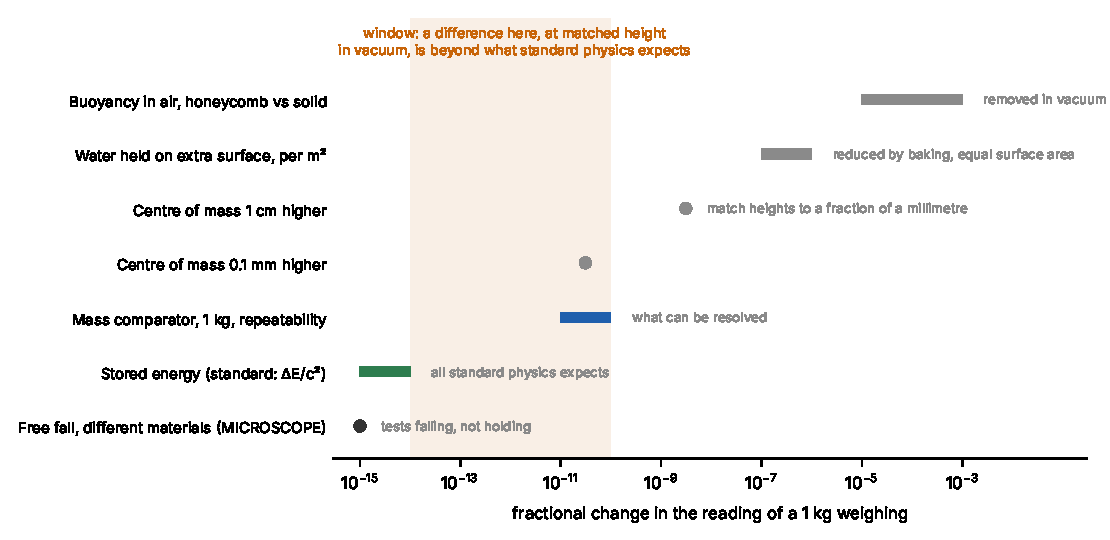
\includegraphics[width=\linewidth]{fig29-1-weighing.pdf}
\caption{Weighing one material in different forms: what the measurement must control, and where a difference would lie beyond the standard account. Air, water held on surfaces and differences in height are each far larger than the window, and are removed by weighing in vacuum, baking, and matching the heights of the centres of mass. Standard physics expects only the energy stored in the structure, $\Delta E/c^2$. A mass comparator resolves about one part in $10^{10}$ to $10^{11}$.}\label{fig:weighing}
\end{figure}

\openm{Which is right has not been tested.} The test is plain: weigh one material, at equal mass, as flat sheets, upright sheets, a honeycomb and a solid block, against each other on a mass comparator. Figure~\ref{fig:weighing} shows what it must control:
\begin{itemize}
\item \textbf{Height.} Weight falls by about three parts in ten million for every metre a body's centre of mass is raised, so the centres of mass must match to a fraction of a millimetre.
\item \textbf{Air.} A honeycomb displaces more air than a solid block, so the weighing is done in vacuum.
\item \textbf{Surface.} A honeycomb has far more surface, and surfaces hold water and gas; the pieces are baked, or made with equal surface area.
\item \textbf{The support.} Each piece is weighed on a mechanical support and on a magnetically levitated one, in case the kind of support matters. Non-magnetic, uncharged material keeps the scale reading one thing.
\end{itemize}
\argm{The standard expectation is far below what a comparator can see.} Rearranging a structure changes the energy it holds by an amount that alters its mass by about one part in $10^{14}$. A difference at one part in $10^{10}$, at matched height in vacuum, would therefore lie beyond anything the standard account expects.

\paragraph{A crystal turned.} Weighing a strongly layered crystal in two orientations tests whether its total weight depends on alignment; a torsion balance tests whether its centre of gravity moves from its centre of mass as it is turned. Highly oriented pyrolytic graphite, whose layers carry heat and charge hundreds of times better along them than across, is the natural specimen. Poynting and Gray searched in 1898 for a directional action between two quartz crystals and found none at the sensitivity of their time.\fn{poynting1899} \argm{Alignment alone shows nothing where it has been tested:} torsion pendulums carrying some $10^{23}$ aligned electron spins show no extra gravitational effect.\fn{heckel2008}

\paragraph{A vibration across a vacuum.} With two crystals in a row and the first set vibrating, the only standard coupling across a vacuum is the gravity of the moving mass, which can be calculated. Any excess at the vibration's frequency would be a transmission through the medium beyond gravity's ordinary form.

\argm{What would count against it:} no difference with structure or orientation at one part in $10^{10}$ would bound how much of the delivery any structure can send anywhere other than the support. It would not touch the account of falling.

\subsection{A spinning body's imprint}\label{sec:spin}

\begin{hypbar}
\textbf{GPT expects:} a spinning body sets the medium around it turning, and the medium carries the spin itself, so a spinning body leaves an imprint beyond what its shape accounts for (Part 16). In Newton's account a uniform sphere's field outside it does not depend on its spin; in General Relativity the spin adds a dragging of order $GJ/c^2r^3$, measured around the Earth by Gravity Probe B,\footnotemark{} and far too small to see around a laboratory rotor.
\end{hypbar}
\footnotetext{\citealp{everitt2011}.}

\openm{The size of the imprint is still owed.} The test is a torsion balance or gravimeter beside a symmetric rotor, compared with the rotor at rest and spun each way. Any signal that follows the spin and not the shape would be the imprint.

\subsection{Clocks and their internal order}\label{sec:clocks}

\argm{Every kind of clock tested is slowed by the same factor:} nuclear, atomic and optical clocks, and the decay of muons, to the precision of each test.\fn{pound1960}\textsuperscript{,}\fn{vessot1980}\textsuperscript{,}\fn{bailey1977} \hypm{In GPT the factor is the medium streaming past every exchange, and is common;} each clock's own rate is set by its structure (Part 18).\fn{rashadaPart18} \openm{No test has compared the slowing of one clock as its internal order is changed:} the same clock, raised the same height, with its internal order altered. The standard account expects no change.

\subsection{Shading at alignments}\label{sec:alignments}

\argm{Gravity is not measurably shielded by matter} (Part 15). A small shading by absorption remains in GPT's account at the scale of the atom, and possibly where bodies line up. \hypm{Eclipses and close alignments are the places to look,} with gravimeters recording through them and the expected tidal signal removed. The standard account expects nothing beyond the tide.

\subsection{Rhythms and the redistribution of delivery}\label{sec:rhythms}

\hypm{Where inside a structured body the medium's delivery lands may depend on its order, and living rhythms may amplify it} (Part 13).\fn{rashadaPart13} Five tests follow:
\begin{itemize}
\item sealed vessels under constant conditions, screened for the lunar tidal periods of 12.42 hours, 13.66 days and 14.77 days, with light and temperature removed;
\item the Moon replaced by a one-tonne lead sphere 0.3 metres away, giving about $7\times10^{-7}$ m/s$^2$, moved on a 12.42-hour cycle;
\item the settling of starch grains in plant cells, compared with the order of the cells around them;
\item biological records matched against superconducting gravimeter records of the same place;
\item the activation record: people's daily rhythms against the Moon's tidal phase at their birth, with the season and cultural effects removed.
\end{itemize}
The standard account expects only the effects of light, temperature and the tide's direct forcing.

\subsection{Re-reading data that exist}

\argm{Several tests need no new instrument.} The Gaia pairs of stars sorted by direction (§\ref{sec:boundary}); gravimeter records through eclipses (§\ref{sec:alignments}); superconducting gravimeter records set beside biological ones (§\ref{sec:rhythms}); and the lunar laser ranging record, which already fixes the Earth and the Moon as carried alike to about one part in $10^{13}$.\fn{williams2012}

\section{Where the Accounts Agree}

Some predictions are often offered as divergences and are not. \argm{GPT and the standard account expect the same here,} and the measurements agree with both:
\begin{itemize}
\item different materials carried alike, to one part in $10^{15}$;
\item light bent alike at every wavelength, and gravitational waves at the speed of light, to one part in $10^{15}$;\fn{abbott2017speed}
\item clocks slowed by height and by speed by the same factors, and particles living longer the faster they move;
\item particle lifetimes changing with height by about one part in $10^{12}$ per ten kilometres, the same in both;
\item Mercury's orbit turned by 43 arcseconds a century (Part 26).\fn{rashadaPart26}
\end{itemize}
These are the outcomes every account must reproduce. They choose between mechanisms only by asking which names what touches what.

\begin{table}[t]\centering\small
\caption{The divergences, with what each account expects and the state of the test.}
\begin{tabularx}{\linewidth}{@{}>{\raggedright\arraybackslash}p{0.22\linewidth} >{\raggedright\arraybackslash}p{0.25\linewidth} >{\raggedright\arraybackslash}p{0.17\linewidth} >{\raggedright\arraybackslash}X@{}}\toprule
\textbf{Test} & \textbf{GPT} & \textbf{Standard} & \textbf{State}\\\midrule
Gravity near $a_0$ & a change of form at the relaxation boundary & Newton; dark matter added & galaxies: one relation; pairs of stars: conflicting\\
Pairs of stars by direction & boundary closer ahead than behind & no difference & data exist; not yet sorted\\
Held weight and structure & may differ & mass alone, $10^{-14}$ & untested at $10^{-10}$\\
Crystal turned & centre of gravity may move & no & untested; quartz null, 1899\\
Spinning body & imprint beyond shape & below reach & untested; size owed\\
Clock, internal order changed & slowing may change & no & untested\\
Alignments & small shading & tide only & gravimeters exist\\
Rhythms & redistribution, amplified & light, heat, tide & five tests proposed\\\bottomrule
\end{tabularx}\label{tab:tests}\end{table}

\section*{Conclusion}
\addcontentsline{toc}{section}{Conclusion}

Most of what is offered as evidence for or against a pressure account of gravity shows the same outcome under both accounts, and can only be decided by asking which names its mechanism. The experiments that can decide are fewer, and sharper. Gravity's change of form near $a_0$ is supported by the galaxies and contested in pairs of stars; GPT adds a test of its own, by direction, in data that already exist. A held body's weight against its structure, a crystal turned, a spinning rotor, a clock with its internal order changed: each is untested, and each is within reach of instruments that exist. Table~\ref{tab:tests} gathers them. Each is stated so that a result can count against GPT, and that is what makes them tests.

\clearpage
\section*{Changes in the Second Edition}
\addcontentsline{toc}{section}{Changes in the Second Edition}

This list records what changed from the first edition and why. Changes to the argument alter what the paper claims or how it supports a claim; clarifications improve wording, sources or presentation and leave the argument as it was.

\subsection*{Changes to the argument}
\begin{itemize}
\item \textbf{The paper's purpose is changed.} The first edition presented its demonstrations as validations already in hand. This edition separates three kinds of difference (the same outcome read two ways, an effect the standard account does not address, a different number) and states that only the last two can be settled by experiment.
\item \textbf{The demonstrations are read again} (Table~\ref{tab:demos}). Kept as readings of the same outcome: the robot arm, the magnet and washer, the balloon in a falling lift, tension, the comb, the gyroscope, the steel plate. Withdrawn as divergences, because their outcomes are measured to be the same under both accounts: the tilt of a quartz-and-foam body in a fall, the earlier motion of dense over loose bodies, the delayed response of hollow spheres in a fall, the rotation of an L-shaped body in a vacuum, apparent mass from heating beyond $\Delta E/c^2$, rising holding cost as fatigue, a magnet's flip changing the gravity around it, and coherent shielding beyond the measured bounds.
\item \textbf{Restated as tests:} the angular weight shift as a crystal's centre of gravity turned in a torsion balance; hollow against solid as the weighing of one material in different forms, held rather than dropped; corridors of crystals as a vibration across a vacuum; the rotating mass as the rotational imprint beyond shape.
\item \textbf{Added from the revised parts:} the relaxation boundary and the pairs of stars, with GPT's own test by direction (Parts 9 and 16); falling and holding as different acts (Part 15); clocks with their internal order changed (Part 18); shading at alignments (Part 15); the five tests of rhythms and redistribution (Part 13); the re-reading of existing data; and what would count against GPT for each.
\item \textbf{Where the accounts agree} is added, so that shared predictions are not offered as divergences.
\end{itemize}

\subsection*{Clarifications}
\begin{itemize}
\item The subtitle changes from \emph{Empirical Foundations of Graviton Pressure Theory} to \emph{Where the Accounts Part Ways, and How to Tell Them Apart}.
\item ``Validation'' is replaced by the expected result, the standard expectation and the state of the test. ``Permission'', ``corridor entry'' and ``coherence alignment'' as causes of motion are replaced by the terms of Parts 5 to 22.
\item One figure and two tables are added; sources are added for each measurement.
\end{itemize}

\bibliography{part29}
\end{document}
